\section{РАЗРАБОТКА ПРОГРАММНЫХ МОДУЛЕЙ}
\label{sec:development}
При разработке системы одними из наиважнейших требований к исходному коду являются его расширяемость и поддерживаемость. Реализация программных модулей с учетом этих требований приводит к простоте расширения функционала в критических местах, обеспечению разделенности и независимости компонентов системы, что улучшает их тестируемость и в целом позволяет добиться реализации более стабильной и простой в понимании кодовой базы.

\subsection{Слой Child-Sum Tree LSTM}
Итак, задача модели Child-Sum Tree LSTM в том, чтобы применить слой Tree LSTM к дереву, обходя его последовательно от литьев к корню. На каждом этапе слой принимает на вход плотный вектор входного слова и набор векторов состояний дочерних узлов синтаксического дерева. Плотный вектор слова это постоянный параметр, в то время как вектора дочерних узлов могут и отсутствовать. Таким образом необходимо выполнять вычисления только для тех узлов, для которых уже известны значения состояний их дочерних узлов.

Затем, после того как рассчитан плотный вектор, соответствующий всему предложению, необходимо найти разницу между полученным значением, и эталонным значением. Эта разница выражается функцией потерь. Значение потерь необходимо минимизировать. Поэтому производится оптимизация функции потерь, экстремум функции потерь в зависимости от обучаемх параметров модели. Затем параметры модели изменяются таким образом, чтобы уменьшить среднее значение функции потерь. Данный процесс отображен на рисунке~\ref{fig:dev:slide}.

\begin{center}
  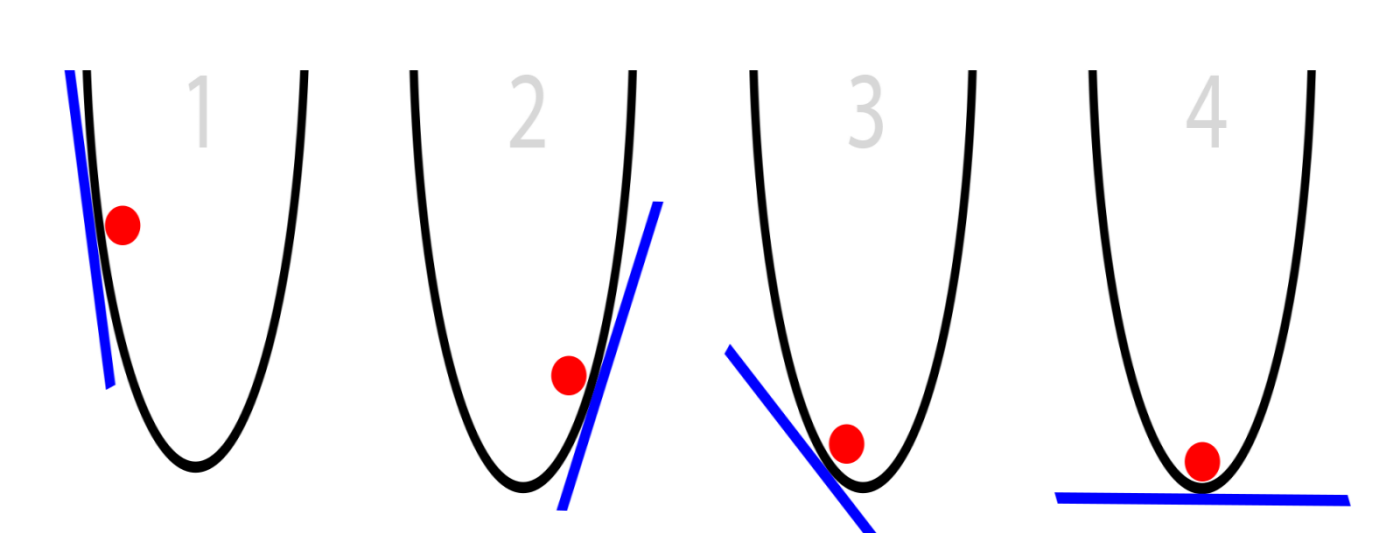
\includegraphics[height=6cm]{sliding_gradient.png}
  \captionof{figure}{Демонстрация оптимизации функции\cite{Goodfellow-et-al-2016}}\label{fig:dev:slide}
\end{center}

Очевидно, что это очень сложный вычислительный процесс, поэтому часто в машинном обучении приходят к оптимизации вычислений на графических процессорах. Для этого в проекте был использован фреймворк Tensor\-flow, позволяющий оптимизировать вычисления на графических процессорах.

Проблема в том, что графический процессор работает с собственным устройством памяти. На рисунке~\ref{fig:dev:cpu_gpu_mem} показана схема перемещения данных между процессорами. Если передавать графическому процессору только математические операции, а все управление производить с помощью центрального процессора, то ускоренные математические вычисления могут и не дать общего прироста производительности, за счет потерь при перемещении данных с одного устройства памяти на другое. С другой стороны, если передать целиком управление графическому устройству, то это очень сильно усложнит процесс разработки. Так как разработчику доступена только оперативная память центрального процессора, то будет возможность только увидеть результат вычислений на графическом процессоре. Промежуточные результаты вычислений и отладка недоступны.

\begin{center}
  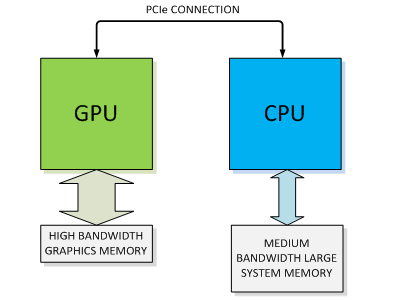
\includegraphics[height=8cm]{cpu_gpu_mem.png}
  \captionof{figure}{Схема перемещения данных в вычислениях на графических процессорах\cite{Goodfellow-et-al-2016}}\label{fig:dev:cpu_gpu_mem}
\end{center}

Tensorflow представляет разработчику высокоуровневое API keras, а управление в большей степени производит самостоятельно. Итак, класс \texttt{cst\-lstm.ChildSumTreeLSTM} является наследником класса \texttt{keras.Layers.Model}. Таким образом класс ячейки Child-Sum Tree LSTM становится одним из блоков Tensorflow и контролируется фреймворком. Алгоритм вычислений, которые производит модель, задан в перегруженной функции \texttt{call}, код которой указан ниже:
\medskip
\begin{lstlisting}[style=Python]
  def call(self, inputs, *args, **kwargs):
    input_word, child_c, child_h = inputs
    child_h_sum = tf.reduce_sum(child_h, 0)
    concat = tf.concat([input_word, child_h_sum], 1)
    i, o, u = tf.split(self.iou_signals(concat), 3, axis=1)
    i, o, u = tf.sigmoid(i), tf.sigmoid(o), tf.tanh(u)
    f = self.forget_signals(child_h) + self.input_transform(input_word) + self.forget_bias
    f = tf.sigmoid(f)
    c = (i * u) + tf.reduce_sum(f * child_c, 0)
    h = o * tf.tanh(c)
    return c, h
\end{lstlisting}
\medskip

Для удобства вычилсений произведены приобразование рассчетов состояний нейронов в узле Child Sum Tree LSTM следующим образом:
\begin{gather}
  \label{eq:func:lstm:i}
  i_{jk} = \sigma(W^{(i)}\cdot{x_j} + U^{(i)}\cdot{\tilde{h_j}} + b^{(i)}) = \sigma({V^{(i)}\cdot{
      \begin{bmatrix}
        x_j\\
        h_j
      \end{bmatrix}} + b^{(i)}}),\\
  \label{eq:func:lstm:forget}
  f_{jk} = \sigma(W^{(f)}\cdot{x_j} + U^{(f)}\cdot{h_k} + b^{(f)}) = \sigma({V^{(f)}\cdot{
      \begin{bmatrix}
        x_j\\
        h_j
      \end{bmatrix}} + b^{(f)}}),\\
  \label{eq:func:lstm:o}
  o_{jk} = \sigma(W^{(o)}\cdot{x_j} + U^{(o)}\cdot{h_j} + b^{(o)}) = \sigma({V^{(o)}\cdot{
      \begin{bmatrix}
        x_j\\
        h_j
      \end{bmatrix}} + b^{(o)}}),\\
  \label{eq:func:lstm:u}
  u_{jk} = \sigma(W^{(u)}\cdot{x_j} + U^{(u)}\cdot{h_j} + b^{(u)}) = \sigma({V^{(u)}\cdot{
      \begin{bmatrix}
        x_j\\
        h_j
      \end{bmatrix}} + b^{(u)}}),\\
  \label{eq:func:lstm:transform}
  c_j = i_j\odot{u_j} + \sum_{k\in{C(j)}}f_{jk}\odot{c_k},
\end{gather}
\begin{explanationx}
\item [где]       $\begin{bmatrix}x_j\\h_j\end{bmatrix}$ --- конкатенация векторов $x_j$ и $h_j$;
\item $V$ --- это конкатенация матриц весов $W$ и $H$.
\end{explanationx}

Параметр \texttt{inputs} представляет собой \texttt{Tuple} в котором хранятся: вектор входного слова, набор векторов состояний ячеек дочерних узлов и набор векторов состояний внутреннего слоя дочерних узлов. Первыя операция и заключается в том, чтобы извлечь из \texttt{inputs} эти три параметра. Такой формат необходим из-за того, что \texttt{cell} --- это перегруженная функция класса предка \texttt{keras.Layers.Model}. Следующий шаг заключается в том, чтобы суммировать состояния внутренних слоев дочерних узлов. Затем, плотный вектор входного слова и данная сумма конкатинируются в один вектор \texttt{concan}. Это позволит вычислить результат одной операцией Tensorflow, куда передастся этот конкатинированный вектор, вместо двух, куда бы передавлася каждый вектор последовательно. Затем, данный вектор \texttt{concat} передается полносвязному слою \texttt{iou\_signals} и результать вычислений разбивается на три равных вертора с помощью функции \texttt{tensorflow.split}. Эти три вектора соответствуют трем сигналам LSTM\@:
\begin{itemize}
\item input сохраняется в переменную \texttt{i};
\item output сохраняется в переменную \texttt{o};
\item update сохраняется в переменную \texttt{u}.
\end{itemize}

Затем к каждому сигналу применяется функция активации. Для input и output функция активации --- это сигмодиа, реализованная \texttt{tensorflow.sig\-moid}, для update --- тангенс, реализованный \texttt{tensorflow.tanh}. Далее строится промежуточная матрица сигнала забывания forget и сохраняется в переменную \texttt{f}. Матрица состояний скрытых слоев дочерних узлов передается в полносвязный слой \texttt{forget\_signals}. Плотный вектор входного слова передается полносвязному слою \texttt{input\_transform}. Каждая строка результирующей матрицы \texttt{forget\_signals} суммируется с выходным вектором \texttt{input\_trans\-form} и к каждому элементу прибавляется \texttt{forget\_bias} --- смещение сигнала забывания.

Затем к промежточной матрице сигнала забывания применяется функция активации сигмоида. Потом получается произведение Адамара данной матрицы с матрицей состояний ячеек дочерних узлов --- \texttt{f * child\_c}. Матрица в результате произведения передается в \texttt{tensorflow.reduce\_sum}, которая сложит все строки матрицы. Затем, произведение Адамара применяется к сигналам input и update. И полученные два вектора складываются и в результате получается состояние ячейки Child-Sum Tree LSTM\@.

Вектор состояния ячейки передается в функцию активации, в данном случае --- тангенс, и результат умножается произведением Адамара на вектор сигнала output. Таким образом будет получен вектор состояния скрытого слоя текущего узла. Состояния скрытого слоя и состояния ячейки вызвращаются из функции.

\subsection{Модель Child-Sum Tree LSTM}
Класс \texttt{cstlstm.ChildSumTreeLSTMClassifier} также является наследником \texttt{keras.Layers.Model}. Поэтому обработка начинается с метода \texttt{call}:
\medskip
\begin{lstlisting}[style=Python]
  def call(self, inputs, training=None, *args, **kwargs):
    out = tf.map_fn(lambda tree: self.eval_tree(json.loads(tree.numpy())), inputs, dtype='int32')
\end{lstlisting}
\medskip

Параметр \texttt{inputs} содержит входные синтаксческие деревья зависимостей, в которых слова заменены индексами их векторов в матрице модели GloVe. Данные синтаксические деревья сохранены в формате JSON, чтобы их можно было лекго упаковать в структуру \texttt{tensorflow.Tensor} с виде строк. Функция \texttt{tensorflow.map\_fn} будет применять переданную ей функцию к каждому элементу переданного в нее тензора. Входной тензор и будет тензор JSON синтаксических деревьев из \texttt{inputs}. Входная функция передана в виде \texttt{lambda} выражения, которое применится для каждого дерева в тензоре. То есть сперва применяется распаковка JSON \texttt{json.loads}, а потом применяется функция обработки деревьев \texttt{eval\_tree}.

Метод \texttt{reset\_metrics} сбрасывает статистику обработанных деревьев для модели:
\medskip
\begin{lstlisting}[style=Python]
  def reset_metrics(self):
    self.loss = 0
    self.result = []
    self.fine = tfe.metrics.Accuracy()
    self.binary = tfe.metrics.Accuracy()
    self.root_fine = tfe.metrics.Accuracy()
    self.root_binary = tfe.metrics.Accuracy()
\end{lstlisting}
\medskip

Функция \texttt{eval\_tree} обрабатывает синтаксическое дерево зависимостей и делает предсказание тональности для отдельных фраз в предложении и для всего предложения целиком. Описание функции представлено ниже:
\medskip
\begin{lstlisting}[style=Python]
  def eval_tree(self, tree, is_root=True):
    sentiment = tree[0]
    word = tree[1][0]
    childs = tree[1][1]
    if word == -1:
      word_embed = tf.random_uniform((self.embed.shape[1],), -0.05, 0.05)
    else:
      word_embed = tf.nn.embedding_lookup(self.embed, word)
    word_embed = tf.reshape(word_embed, (1, word_embed.shape[0]))
    word_embed = self.projection(word_embed)
    word_embed = self.dropout(word_embed)
    child_h = []
    child_c = []
    for child in childs:
      child_state = self.eval_tree(child, is_root=False)
      child_c.append(child_state[0])
      child_h.append(child_state[1])
    if childs:
      child_c = tf.convert_to_tensor(child_c)
      child_h = tf.convert_to_tensor(child_h)
    else:
      child_c = tf.zeros((1, 1, self.encoder.unit_number))
      child_h = tf.zeros((1, 1, self.encoder.unit_number))
    child_state = self.encoder([word_embed, child_c, child_h])
    logits = self.output_layer(child_state[1])
    self._add_metrics(sentiment, logits)
    if is_root:
      prediction = tf.cast(tf.argmax(logits[0]), tf.int32)
      self.result.append(prediction)
      self.root_fine(sentiment, prediction)
      if sentiment != 2:
        self.root_binary(int(sentiment > 2), tf.cast(prediction > 2, tf.int32))
      return prediction
    return child_state
\end{lstlisting}
\medskip

Входной параметр \texttt{tree} содержит дерево зависимостей в формате списка. Параметр \texttt{is\_root} несет информацию о том, является ли текущий узел корнем дерева или нет. Как видно в функции \texttt{call} функция \texttt{eval\_tree} вызывается без параметра \texttt{is\_root}, поэтому ему будет присвое его стандартное значение. Этот ход позволяет скрыть от пользователя функции то, что метод является рекурсивным. Вызовы функции \texttt{eval\_tree} из нее же производятся уже с явным указанием значения \texttt{is\_root}.

Сперва распаковываются значения параметров текущего узла дерева. Эталонное значечние тональности для узла сохраняется в \texttt{sentiment} типа \texttt{int}. Значение индекса плотного вектора соответствующего входному слову сохраняется в переменную \texttt{word}. Список дочерних узлов текущего узла сохраняется в переменную \texttt{childs}.

Переменная \texttt{sentiment} может принимать значения целых чисел в интервале от 0 до 4:
\begin{itemize}
\item 0 --- очень плохая тональность;
\item 1 --- плохая тональность;
\item 2 --- нейтральная тональность;
\item 3 --- хорошая тональность;
\item 4 --- очень хорошая тональность.
\end{itemize}

Затем происходит поиск соответстующего плотного вектора по заданному индексу. Если значения индекса \texttt{word} равно -1, то слово не было найдено в модели GloVe, и плотный вектор будет генерироваться случайным образом. Для этого применяется функция \texttt{tensorflow.random\_uniform}, которая сгенерирует вектор, соответствующией модели GloVe размерности, которая хранится в поле \texttt{embed}. Элементы вектора будут равномерно распределены в интервале от -0.05 до 0.05. Если же слово присутствует в модели GloVe, то применяется функция \texttt{tensorflow.nn.embedding\_lookup}, которая вернет соответствующий вектор из модели GloVe.

Затем к полученному плотному вектору прменяется функция \texttt{tensor\-flow.reshape}. Эта функция добавит тензору одно измерение. То есть плотный вектор будет помещен в вектор, и будет там единственным элементом. Требование реализации полносвязных слоев в keras заключается в том, что минимальная размерность входного вектора равняется двум.

Итак, полученная матрица передается в полносвязный слой проекции GloVe \texttt{projection}. Далее результат передается в слой исключения \texttt{dropout}. Затем, переменные \texttt{child\_h} и \texttt{child\_c} инициализируются пустыми списками.

Затем в цикле перебираются все элементы из списка \texttt{childs}. Для каждого из них получают значение плотного вектора, кодирующего семантику фразы, сответствующей дочернему узлу, с помощью рекурсивного вызова функции \texttt{eval\_tree}. В этот раз параметр \texttt{is\_root} явно инииализируется значением \texttt{False}. Результаты состояний ячейки и скрытого слоя добавляются в списки \texttt{child\_c} и \texttt{child\_h}.

После того как значения состояний для дочерних узлов собраны, списки Python приводятся к типу \texttt{tensorflow.Tensor} с помощью функции \texttt{ten\-sorflow.convert\_to\_tensor}. Если же у текущего узла нет дочерних узлов, то есть он является листом в дереве, то для него генерируются тензоры состояний дочерних узлов с помощью функции \texttt{tensorflow.zeros}. Полученные тензоры будут по размерности совпадать с тензором состояния для узла с одним дочерним узлом, и будут проинициализированы нулями.

Далее, в список упаковываются:
\begin{itemize}
\item плотный вектор входного слова \texttt{word\_ember};
\item тензор состояний ячеек дочерних узлов \texttt{child\_c};
\item тензор состояний скрытых слоев дочерних узлов \texttt{child\_h}.
\end{itemize}

Полученный список передается в слой Child-Sum Tree LSTM \texttt{encoder}. Для полученного вектора состояния скрытого слоя делается предсказание классификатором \texttt{output\_layer}. Затем вызывается метод \texttt{\_add\_metrics}, куда передается полученное предсказание тональности \texttt{logits} и эталонное значение тональности \texttt{sentiment}. Этот метод сохранит информацию о том, было ли пресказание успешным, чтобы потом вычислить точность работы модели.

Затем, если рекурсия находится в итерации корневого узла дерева, то необходимо добавить информацию о точности модели в рамках рассчета метрики предсказаний тональности предложений, а не только отдельных фраз и слов. В \texttt{prediction} сохраняется приведенный в \texttt{int32} результат вычисления функции argmax реализованной в \texttt{tensorflow.argmax}. Это равняется индексу максимального значения в векторе предсказаний \texttt{logits[0]}. Данный процесс соответствует алгоритму классификатора softmax. В список предсказаний \texttt{result} добавляется полученное значения. В список \texttt{root\_fine} добавляются полученное значение вместе с эталонным, чтобы потом рассчитать точность модели на предсказаниях тональности предложения. Затем, если эталонное значение тональности не равняется нейтральному, то будет собрана информация о бинарном предсказании. В качестве эталона будет хранится приведенное к \texttt{int} значение \texttt{sentiment > 2}. В качестве предсказания так же будет хранится результат сравнение полученного ранее предсказания с двойкой. Полученное предсказание возвращается из функции.

Для не корневого узла из функции будут возвращаться состояния скрытого слоя и ячейки Tree LSTM, так как это часть рекурсивного обхода дерева.

\subsection{Обучение модели}
Обучение модели описано в классе \texttt{train.Train}. Его метод \texttt{eva\-lua\-te\_dataset} реализует обработку набора данных. Код метода представлен ниже:
\medskip
\begin{lstlisting}[style=Python]
  def evaluate_dataset(model, trees, batch_size=25):
    model.reset_metrics()
    complicity = 0
    for batch in tfe.Iterator(trees.shuffle(buffer_size=12000).batch(batch_size)):
      model(batch)
      complicity += batch_size
      trees.print_progress_bar(complicity)
      metrics = {name: metric.result().numpy() * 100 for name, metric in zip(["fine", "binary", "root_fine", "root_binary"], [model.fine, model.binary, model.root_fine, model.root_binary])}
    return ' '.join(['\%s: \%.2f' \% (name, metric) for name, metric in metrics.items()])
\end{lstlisting}
\medskip

Сперва информация о прошлых вызовах модели стирается вызовом метода \texttt{reset\_metrics}. После этого инициализируется переменная \texttt{complicity}, которая хранит прогресс обработки набора данных. Для итерации по набору данных используется \texttt{tensorflow.contrib.eager.Iterator}, который предоставляет самый производительный метод обхода наборов данных. Прежде чем начать итерации по набор данных к нем применяется функция \texttt{tenosr\-flow.data.TextLineDataset.shuffle}, которая будет перемешивать деревья в наборе данных. Затем перемешанный набор данных делиться на группы размером \texttt{batch\_size}.

Каждую итерацию модель Child-Sum Tree LSTM применяется к группе деревьев \texttt{batch} из набора данных. Инкрементируется переменная завершенности обработки на размер группы. После того как набор данных обработан, вычисляются точности модели согласно различным параметрам и возвращается строка с выводом об успехах модели при выполнении набора данных.

Метод \texttt{train\_epoch} класса \texttt{train.Train} реализует эпоху обучения модели Child-Sum Tree LSTM\@. Код метода представлен ниже:
\medskip
\begin{lstlisting}[style=Python]
  def train_epoch(model, train_trees, model_optimizer, embedding_optimizer, batch_size=25):
    train_loss = 0
    model.reset_metrics()
    complicity = 0
    for batch in tfe.Iterator(train_trees.shuffle(buffer_size=12000).batch(batch_size)):
      with tfe.GradientTape() as tape:
        tape.watch(model.variables)
        model(batch)
      gradient = tape.gradient(model.loss, model.variables)
      embed_grads = gradient[:len(model.embed_variables)]
      model_grads = gradient[len(model.embed_variables):]
      train_loss += model.loss
      model_optimizer.apply_gradients(zip(model_grads, model.model_variables), global_step=tf.train.get_global_step())
      embedding_optimizer.apply_gradients(zip(embed_grads, model.embed_variables), global_step=tf.train.get_global_step())
      complicity += batch_size
      train_trees.print_progress_bar(complicity)
    print('\n')
    return train_loss
\end{lstlisting}
\medskip

Сперва инициализируется значение суммарной функции потерь \texttt{tra\-in\_loss}. Сбрасываются все метрики с помощью вызова \texttt{reset\_metrics}. Затем значение завершенности эпохи \texttt{complicity} также инициализируется нулем.

Тренировочный набор данных случайным образом перемешивается с помощью вызова \texttt{shuffle}, и делится на группы размером \texttt{batch\_size} с помощью вызова \texttt{batch}. Создается итератор по группам деревьев в перемешанном наборе данных с помощь \texttt{tensorflow.contrib.eager.Iterator}, и начинается последовательный обход всего набора данных.

Итерация начинается с создания \texttt{tensorflow.contrib.eager.Gradi\-entTape} в виде менеджера контекста. После того как интерпретатор Python покинет блок менеджера контекста, объект \texttt{tape} будет исправно закрыт. Внутри блока в метод \texttt{tape.watch} передаются все тренируемые параметры модели Child-Sum Tree LSTM\@, полученные с помощью дескриптора \texttt{variables}. Это позволит объекту \texttt{tape} вычислить градиент для модели относительно этих параметров модели. Затем модель выпоняется для текущего набора данных

Далее вычисляются функции потерь для параметров модели с помощью вычисления значения градиента. Для этого в \texttt{tape.gradient} передается функция потерь модели, рассчитанная на выходе Child-Sum Tree LSTM\@. Полученные потери разбиваются на два списка: \texttt{embed\_grads} и \texttt{model\_grads} соответственно потери для параметров слоя проекции модели GloVe и для остальных параметров модели. После этого потери для текущей группы прибавляются к суммарным потерям эпохи обучения.

После того ка потери вычислены, они передаются оптимизаторам. Объект \texttt{model\_optimizer} оптимизирует параметры всей модели, кроме параметров слоя проекции GloVe, которые будет оптимизировать \texttt{embedding\_optimi\-zer}. Затем инкрементируется счетчик завершенности модели \texttt{complicity}. Затем обновляется строка состояния. После того как все группы обработаны, вввозвращаются суммарные потери всей эпохи обучения \texttt{train\_loss}.

Загрузка модели GloVe реализована методом \texttt{load\_embeddings}:
\medskip
\begin{lstlisting}[style=Python]
  def load_embeddings(embedding_path):
    """Loads embedings, returns weight matrix and dict from words to indices."""
    print('loading word embeddings from \%s' \% embedding_path)
    weight_vectors = []
    word2index = {}
    with codecs.open(embedding_path, encoding='utf-8') as f:
      for line in f:
        word, vec = line.split(u' ', 1)
        word2index[word] = len(weight_vectors)
        weight_vectors.append(np.array(vec.split(), dtype=np.float32))
        word2index[u'-LRB-'] = word2index.pop(u'(')
        word2index[u'-RRB-'] = word2index.pop(u')')
     weight_vectors.append(np.random.uniform(-0.05, 0.05, weight_vectors[0].shape).astype(np.float32))
     return np.array(weight_vectors, dtype=np.float32), word2index
\end{lstlisting}
\medskip

В первую очередь выводится строку состояния. Затем инициализируется список плотных векторов \texttt{weight\_vectors}. После него инициализирется словарь соответствий слов индексам их векторов в матрице модели GloVe. Далее открывается менеджер контекста для файла модели GloVe, с кодировкой \texttt{utf-8}. После этого последовательно читаются все строчки из файла. Каждая строчка разбивается по пробелу на две части, первая содержит слово и сохраняется в переменную \texttt{word}, вторая --- плотный вектор и сохраняется в переменную \texttt{vec}. Далее в \texttt{word2vec} добавляеся запись о текущем слове и о соответствующем ему индексу. В список плотных векторов добавляется новый вектор. Затем символы \texttt{-LRB-} и \texttt{-RRB-} заменяются на символы левой и правой скобки соответственно.

В конце, генерируется случайный вектор, который будет соответствовать всем словам, отсутствующим в модели GloVe. Данный вектор добавляется в список плотных вектов. Функция возвращает список плотных векторов, приведенный к матрице, и словарь \texttt{word2index}.